\documentclass[a4paper]{scrartcl}
\usepackage[utf8]{inputenc}
\usepackage[english]{babel}
\usepackage{graphicx}
\usepackage{lastpage}
\usepackage{pgf}
\usepackage{wrapfig}
\usepackage{fancyvrb}
\usepackage{fancyhdr}
\usepackage{float}
\pagestyle{fancy}

% Create header and footer
\headheight 27pt
\pagestyle{fancyplain}
\lhead{\footnotesize{Data Storage Paradigms, IV1351}}
\chead{\footnotesize{Project Report}}
\rhead{}
\lfoot{}
\cfoot{\thepage\ (\pageref{LastPage})}
\rfoot{}

\title{Project Report Task 2}
\subtitle{Data Storage Paradigms, IV1351}
\author{}
\date{2024-11-21}

\begin{document}

\maketitle
\noindent\textbf{Project members:} \\ \hfill
Jonathan Värild, varild@kth.se \\ \hfill
Oscar Caddeo, ocaddeo@kth.se \\ \hfill
Elias Holm, eliholm@kth.se \\ \hfill

\section*{Declaration:}

By submitting this assignment, it is hereby declared that all group members listed above have contributed to the solution. It is also declared that all project members fully understand all parts of the final solution and can explain it upon request.

It is furthermore declared that the solution below is a contribution by the project members only, and specifically that no part of the solution has been copied from any other source (except for lecture slides at the course IV1351), no part of the solution has been provided by someone not listed as a project member above, and no part of the solution has been generated by a system.

\section{Introduction}


\section{Literature Study}


\section{Method}

\section{Result}

\begin{figure}[H]
  \begin{center}
    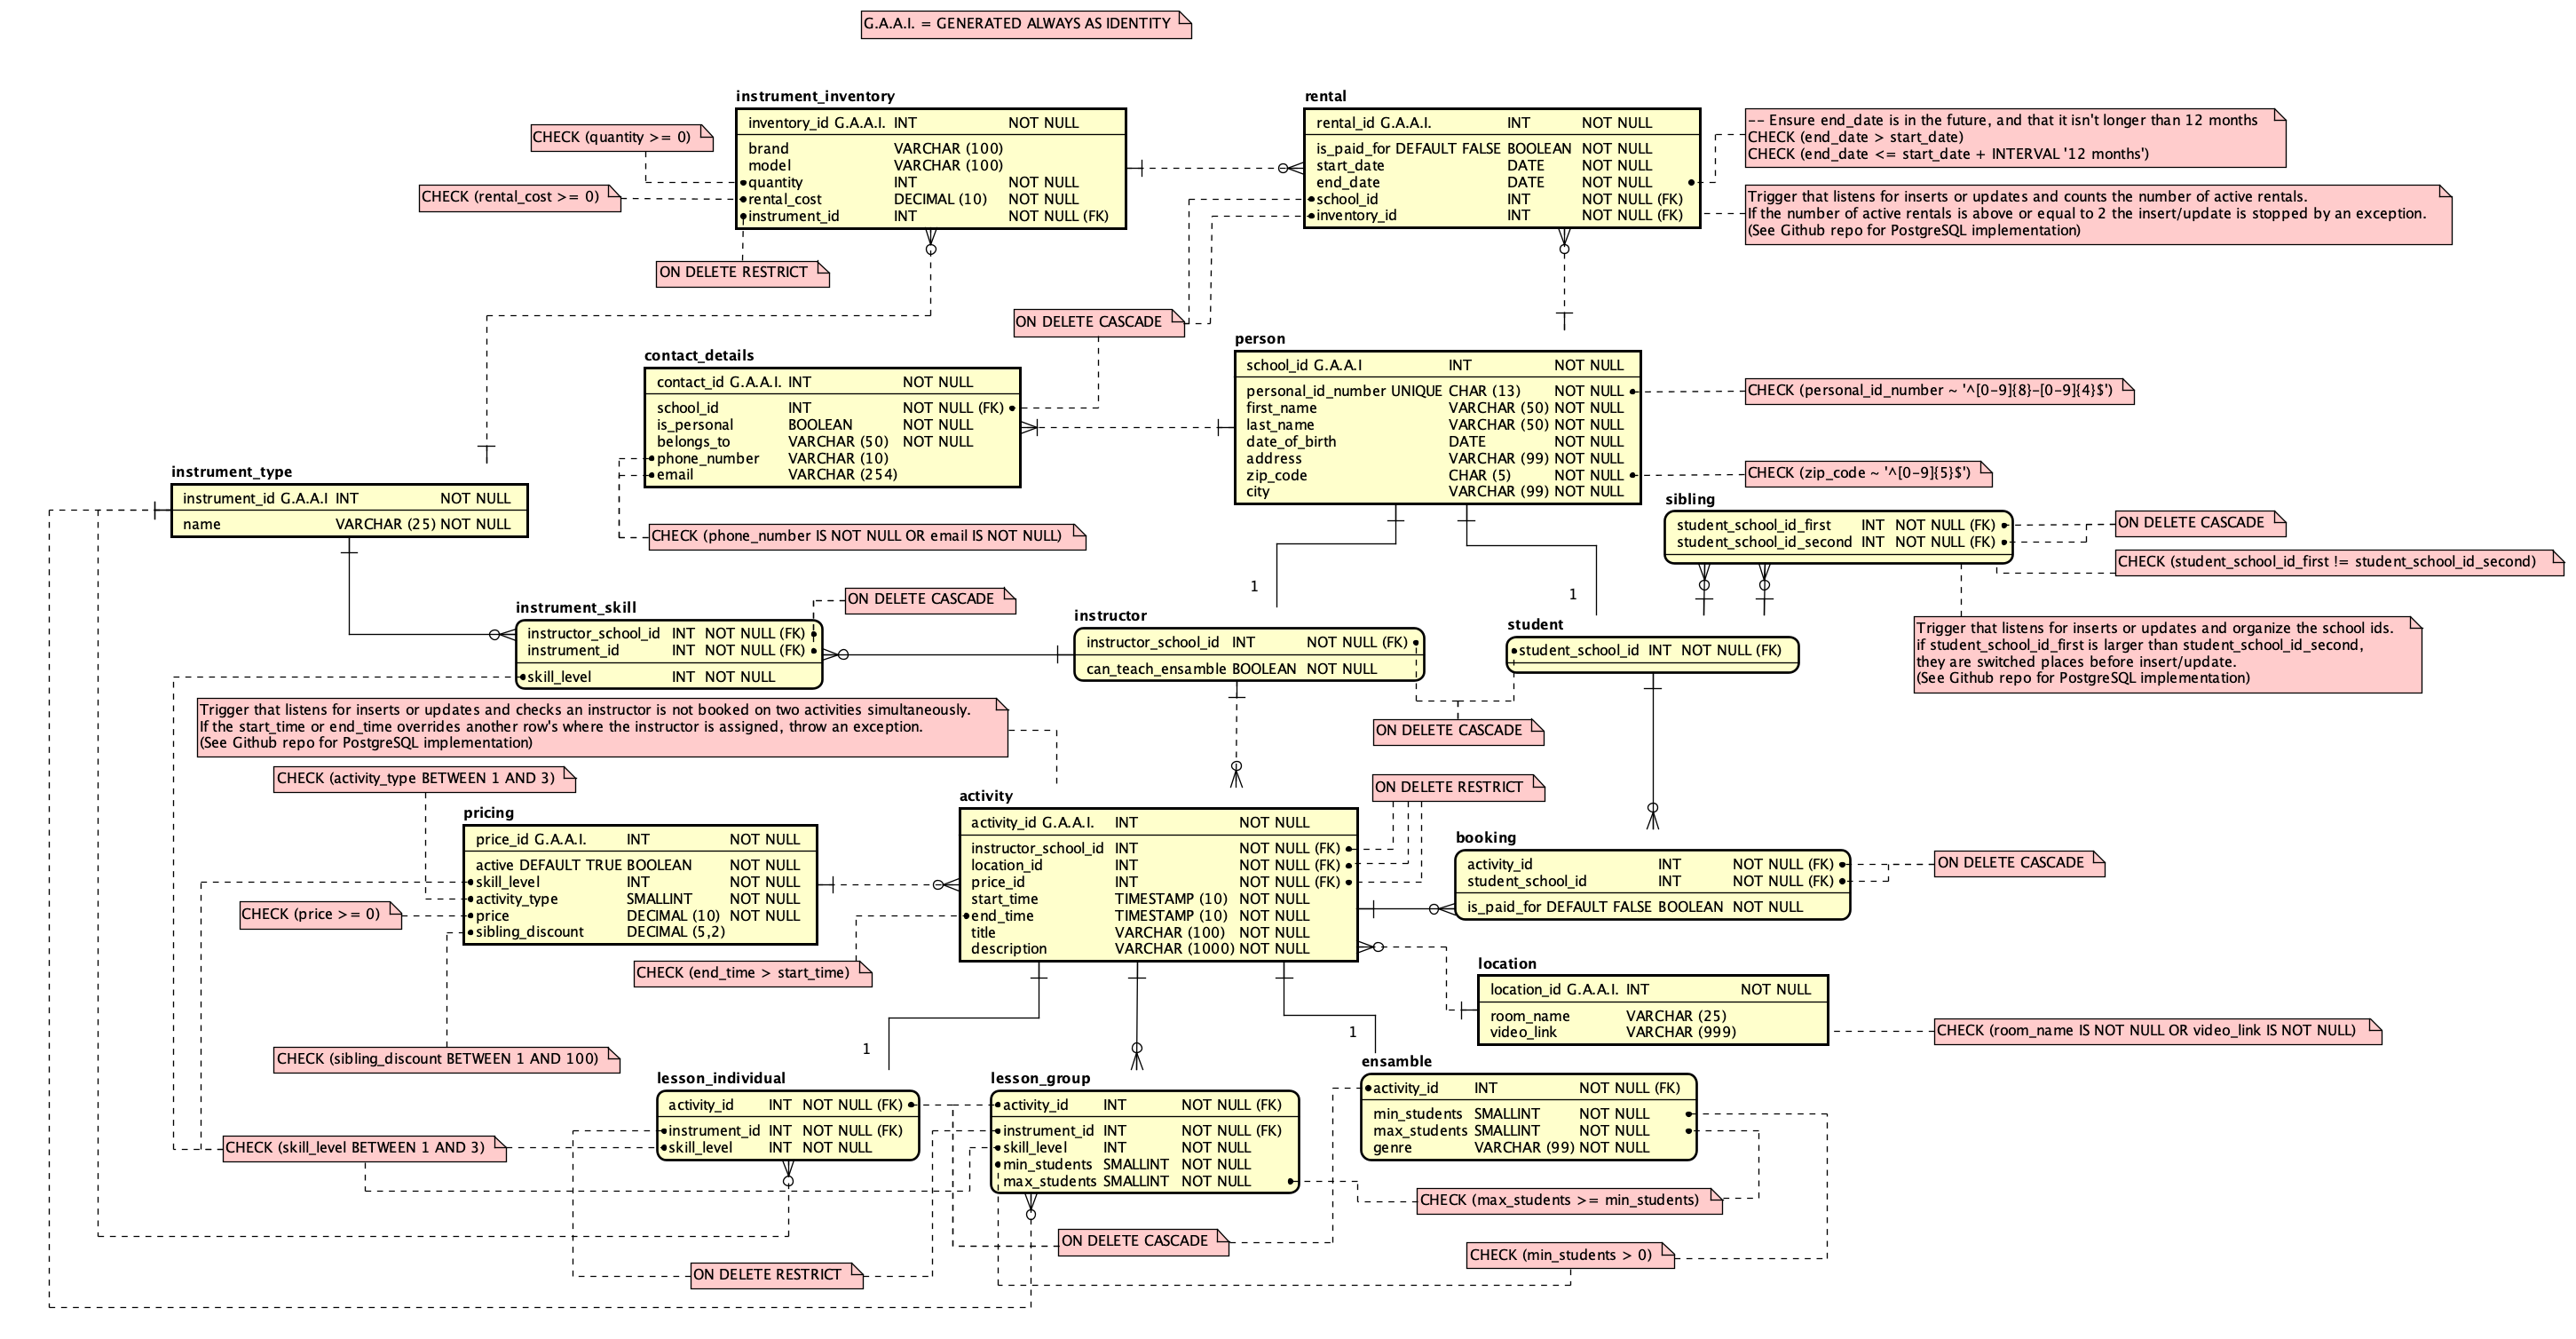
\includegraphics[scale=0.12]{Diagram Picture.png}
    \caption{The physical/logical diagram that we came up with.}
    \label{fig:diag}
  \end{center}
\end{figure}

\section{Discussion}

\subsection{Question 1}

\subsection{Question 2}

\subsection{Question 3 ...}

\section{Comments About the Course}


\end{document}
